\subsubsection{Mergesort}
Mergesort is a well-known sorting algorithm based on the Divide$\&$Conquer paradigm. Thinking to a parallel version of Mergesort is therefore quite natural. First of all, $S$ is scattered among the $N$ processes. Each process locally sorts its own portion of $\frac{n}{N}$ elements, using a standard sequential sorting algorithm, like \textit{qsort}. At this point, a sequence of $\lceil \log_{2}{N} \rceil$ steps starts; in everyone of them, a \textit{distribution} phase precedes a \textit{merging} phase. The distribution phase is performed \textit{between different processes}: for instance, $rank$ $1$ sends its data to $rank$ $0$, while $rank$ $3$ to $rank$ $2$ and so on. On the other hand, the merging phase is done locally by all the processes that received a portion of data. Figure~\ref{merge-dist} clarifies these concepts. Further, we observe that as its sequential counterpart, our version of mergesort needs an auxiliary array of size $n$. 
\begin{algorithmic}[1]  
	\medskip
	\STATE $Scatter( S, S\_local )$
	\STATE $qsort( S\_local )$
	\REPEAT 
		\STATE $distribution( S\_local )$
		\STATE $fusion ( S\_local )$
	\UNTIL $i < \log_{2}{N}$
	\medskip
\label{alg1}
\end{algorithmic}
Notice that steps $\lbrace 1, 2 \rbrace$ will be typically performed by all our algorithms, not just by Mergesort. We conclude this overview by emphasizing that the \textit{distribution} of data in each step can be handled in many different ways; that is, there are many possible communication patterns between processes, that may lead to different performance behavior (for instance, because of the change of the load on the interconnection structure) . We will address this important topic in a following section.

\begin{figure}[h]
        \centerline{
               \mbox{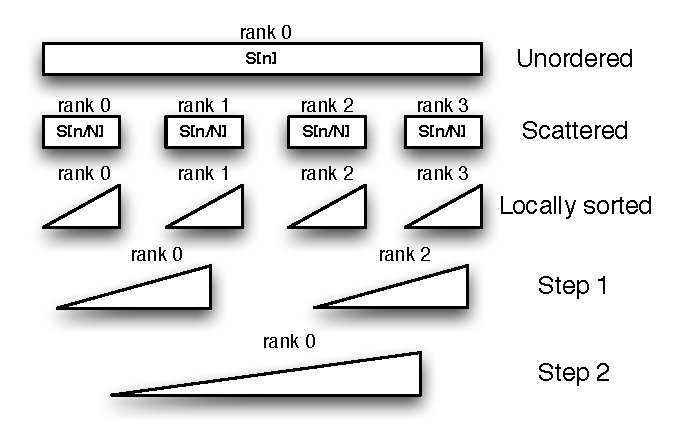
\includegraphics[scale=0.70]{mergesort-pict1}}
        }
        \caption{Parallel mergesort for $N = 4$.}
        \label{merge-dist}
\end{figure}


%\subsubsection{Parallel version}
%Descrizione della parallelizzazione dell'algoritmo; possibile uso di pseudocodice. Per lo pseudocodice ho definito in Relazione.tex un template da poter utilizzare. Ad esempio, se voglio includere lo pseudocodice del mergesore, basta scrivere: $lstinputlisting{mergesort.code}$. Per convenzione i file con lo pseudocodice scriviamoli con estensione .code.
%\subsubsection{Mapping virtual processors onto different cores} 
%only if they are considered in the specific version
%\subsubsection{Performance Analisys} 
%Qua discutiamo di completion time e quindi scalability ecc. Magari facciamo un confronto con quelle che devono essere le prestazioni ideali.
%\subsubsection{Efficiency} 
%Magari il nome di questa sezione va ''raffinato''..cmq, qua discutiamo di quello che diceva il coppola, cioè ad ogni step dell'ordinamento quanto riusciamo a sfruttare l'architettura parallela. Magari c soffermiamo su quanto la presenza del multicore sia effettivamente sfruttata e quanto. 
%\subsubsection{statistical analysys}
%to be discussed in case variance is high...questo magari possiamo scriverlo DOPO aver fatto i test.
